% Capítulo 3
\chapter{Revisão do Estado da Arte}
\label{cap:cap3}

Este capítulo busca compreender o estado da arte e identificar desafios e oportunidades de pesquisa sobre a implementação de mecanismo \textit{throttling}, especialmente no contexto de dispositivos \acs{IoT} presentes na computação dirigia à energia (\acl{EDC}). Assim, foi realizado uma pesquisa sobre a aplicação de fatores limitantes e os motivadores da atuação desse mecanismo.


\section{Protocolo}
Para esta revisão, adotaram-se práticas descritas no método apresentado por \citeauthor{kitchenham_systematic_2009} (\citeyear{kitchenham_systematic_2009}), mas decidiu-se por não utilizar uma revisão sistemática como protocolo. Assim, a captação dos estudos foi realizada através da aplicação da técnica de \textit{snowballing}, que é capaz de expandir a base de referências e viabilizar a identificação de padrões recorrentes, aprofundando a compreensão no tema de estudo.

O processo de \textit{snowballing} é descrito como abordagem iterativa de busca por referências em revisões de literatura \cite{wohlin_guidelines_2014}. Seu método é caracterizado através das iterações onde em cada uma é realizado análise sobre as referencias citadas nos artigos seminais (\textit{backward}) e também dos estudos que utilizaram esses artigos como referencia (\textit{forward}). Portanto, neste trabalho a abordagem de \textit{snowballing} foi executada em iterações, aplicando ambos os métodos (\textit{backward} e \textit{forward}). Os trabalhos resultantes de cada iteração  foram incluídos com base nos critérios de seleção previamente definidos na Subseção \ref{cap3:criteriosinclusaoexclusao}.




\subsection{Critérios de inclusão e exclusão} 
\label{cap3:criteriosinclusaoexclusao}

Tendo em vista a necessidade de realizar filtragem no material encontrado durante iterações, foram adotados critérios de inclusão e exclusão como já previsto no método em  \cite{wohlin_guidelines_2014}. Assim, os estudos resultantes foram obtidos com base nos critérios definidos com a intenção de cobrir o maior numero de trabalhos relacionados ao tema de pesquisa e ao mesmo tempo evitar os trabalhos com base nos critérios estabelecidos.

Portanto, os critérios de exclusão utilizados podem ser vistos descritivamente na Tabela \ref{table:cap3:criterios}. Estes critérios foram definidos para assegurar que apenas os estudos que se relacionassem com a pesquisa fossem incluídos, evitando artigos segundo os critérios ja apresentados.


\begingroup
\begin{table}[htbp]
	
	\centering
	\caption{\textit{Snowballilng}: Critérios de Exclusão.}
	%	\small
	%	\tabcolsep=0.05cm
	\begin{tabular}{ l | l  }
		\hline
		 \multicolumn{2}{c}{Critério de Exclusão}  \\
		\hline\addlinespace[1pt]
		CE-1	& Não escrito em inglês. \\
      	CE-2	& Sem aderência aos eixos temáticos. \\
		CE-3	& Sem indícios diretos com às questões de pesquisa.\\
		CE-4	& Artigos derivações do mesmo autor  ou resumo.\\
		CE-5	& Tutoriais, Capítulos de livros e Relatórios técnicos (Literatura Cinza).\\
		CE-6	& Trabalhos duplicados.\\
		CE-7	& Artigos não disponíveis integralmente para leitura.\\
		CE-8	&  Artigos predecessores à revisão seminal.\\
		\hline\addlinespace[2pt]
	\end{tabular}
	\label{table:cap3:criterios}
	\\
	\footnotesize Fonte: elaborado pelo autor.
	
\end{table}
\endgroup

\subsection{Processo}

Para selecionar os estudos que formam a base do trabalho foi utilizada a base bibliográfica SciVerse Scopus
\footnote{Plataforma acessível em: \url{https://www.scopus.com/}}. A escolha desta plataforma como fonte de informação foi justificada pela capacidade de indexar os principais repositórios acadêmicos para a area de estudo, dentre elas ACM Digital Library, Elsevier, IEEE Xplore, Springer Link, Web of Science entre outras.

O artigo seminal foi selecionado mediante análise de sua influência, impacto e credibilidade para o campo de pesquisa deste estudo. Portanto, utilizando o artigo como único ponto de partida, segue o processo iterativo \textit{snowballing} conforme estabelecido. As etapas podem ser visualizadas na Figura \ref{fig:cap3snowballing} onde é apresentado a visão completa do processo e ações determinadas.


\begin{figure}[H]
	\centering	
	\caption{Processo \textit{Snowballing}.} 
	\label{fig:cap3snowballing}
	\noindent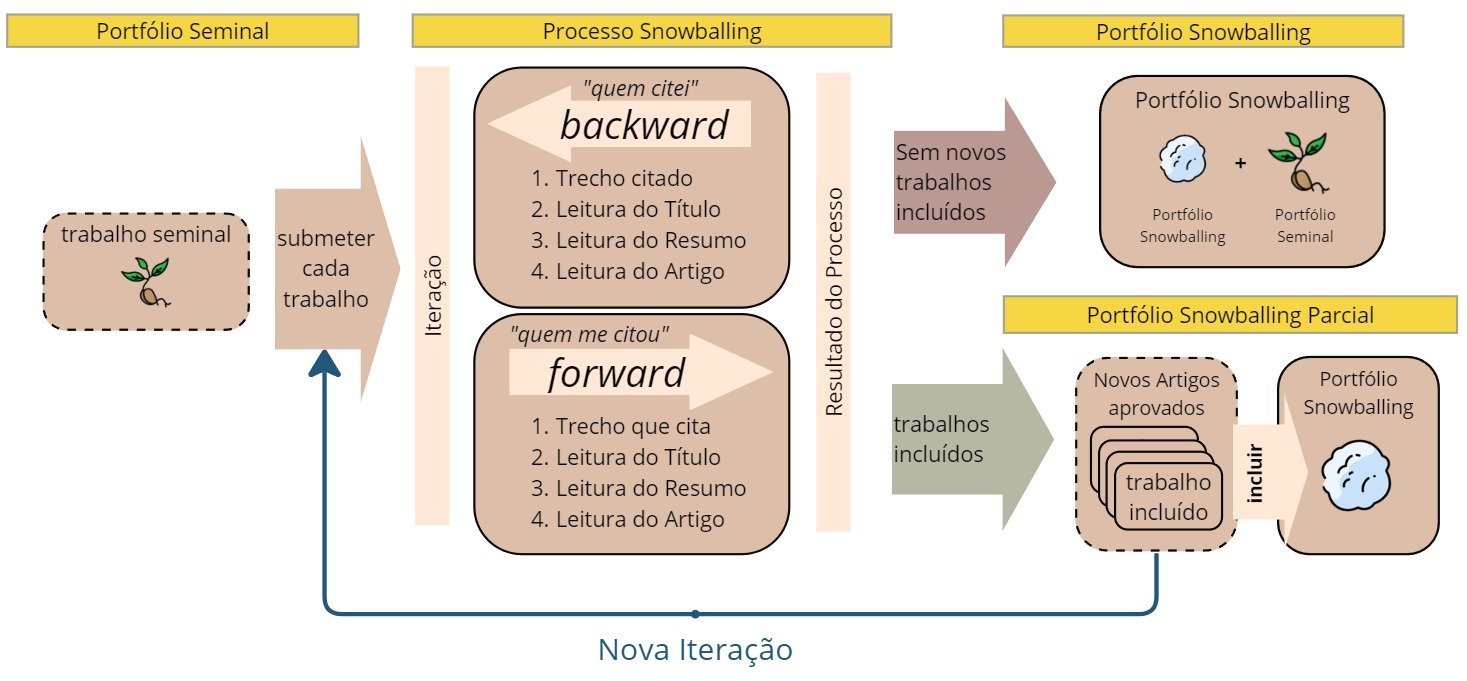
\includegraphics[width=1\linewidth]{Imagens/cap3/snowballing.jpg} 
	
	Fonte: elaborado pelo autor.
\end{figure}

Em cada iteração, são realizadas ações com o objetivo de selecionar os trabalhos considerados relevantes para o estudo. Essas, partem da análise da leitura da parte do texto que foi citado quando em \textit{backward} ou a leitura do trecho que cita quando em \textit{forward}, além da leitura do titulo, resumo e por fim, da leitura integral do trabalho. Assim, ao passo que finalizada interação, teremos os novos artigos que servem como entrada para iteração seguinte. Caso uma iteração finalize sem nenhum novo trabalho adicionado, conclui-se o processo \textit{snowballing}, os resultados são unidos ao artigo seminal em composição ao portfólio final obtido. A Figura \ref{fig:cap3etapassnowballing} apresenta o processo de seleção dos trabalhos avaliados.

\begin{figure}[H]
	\centering	
	\caption{Resultado das Iterações \textit{Snowballing}.} 
	\label{fig:cap3etapassnowballing}
	\noindent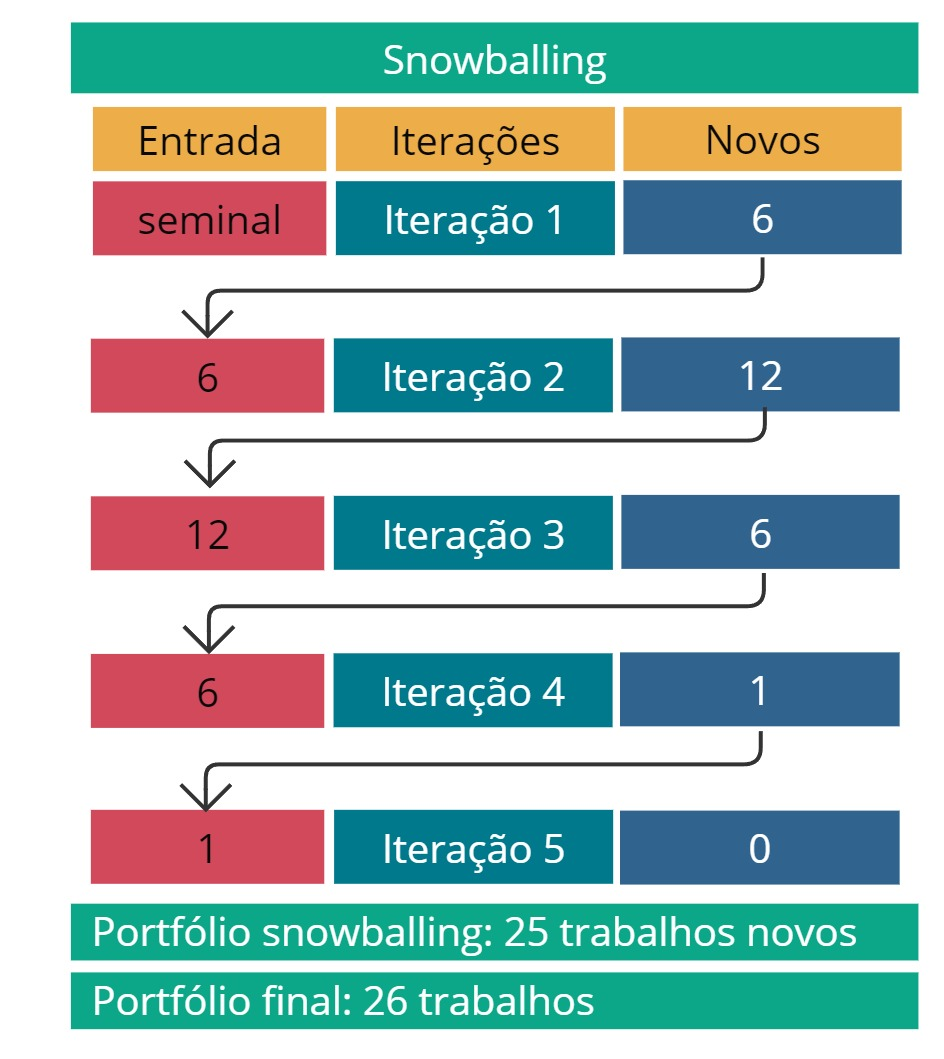
\includegraphics[width=0.7\linewidth]{Imagens/cap3/etapas.jpg} 
	
	Fonte: elaborado pelo autor.
\end{figure}


A dinâmica de inclusão e filtragem de trabalhos relacionados, proporcionou visitar ao todo 1171 trabalhos por método \textit{backward}, além de 3597 trabalhos por \textit{forward} gerando uma cobertura total de 4768 artigos alcançados. É previsto durante o \textit{snowballing} proporcionar rastreabilidade na inclusão dos trabalhos. A Figura apresenta esta característica enquanto proporciona visão sobre os trabalhos mencionados. 

\begin{figure}[H]
	\centering	
	\caption{PENSANDO SE VALE APRESENTAR GRAFO COM A a rastreabilidade dos trabalhos aqui.} 
	\label{fig:cap3etapassnowballing}
	\noindent\includegraphics[width=0.7\linewidth]{example-image} 
	
	Fonte: elaborado pelo autor.
\end{figure}

Finalmente o processo Snowballing proporcionou a criação do portfólio total de artigos composto por 26 trabalhos que serviram como base para o estudo, os resultados obtidos estão descritos na Seção ref{cap3:resultados}.


\section{Resultados}
\label{cap3:resultados}

Foi característico ao portfólio de trabalhos selecionados a apresentação do leitor aos desafios ligados à como os agentes \acs{IoT} com capacidade de coleta de energia, realizam suas funções em detrimento do cenário de restrições energéticas. É recorrente a presença dos mecanismo de ajuste do comportamento dos dispositivos mediante observação de termos que auxiliam ao processo de tomada de decisão sobre como o dispositivo deve atuar diante de um ou outro cenário encontrado.

A lista de artigos pode ser visualizado totalmente na Tabela \ref{table:cap3:trabalhosobservados}, aqui uma visão geral dos trabalhos selecionados pode ser obtida. Todavia, um ponto de destaque é que mesmo os cenários de atuação com uma abordagem transiente, como apresentados por \citeonline{merrett_energy-driven_2017} e \citeonline{sliper_energy-driven_2020}, ainda mantem a necessidade de mecanismos para limitação de gasto energético quando ocorrem os processos de ajuste a potencia energética administrada ao dispositivo. 

%falar sobre todos os trabalhos mencionam ajustes de comportamento para estar compativel com gasto energético.


\begingroup
\begin{table}[ht]
	\centering
	\caption{ Trabalhos observados.}
	\smaller[1]
	\tabcolsep=0.15cm
	\rowcolors{1}{gray!78}{white}
	\begin{tabular}{cp{11cm}c}
		\toprule
		ID &  Titulo & Tipo \\\midrule
		SB0-0001 &	Power Management in Energy Harvesting Sensor Networks & Periódico \\
		SB1-0001 &	 Energy-Driven Computing: Rethinking the Design of Energy Harvesting Systems & Conferência\\
		SB1-0002 &	 Lightweight operation scheduling for self-powered IoT devices  & Conferência \\
		SB1-0003 & Adaptive operating mode management model for efficient energy harvesting systems & Periódico\\
		SB1-0004 &	Energy Management in Wireless Sensor Networks: A Survey  &\\
		SB1-0005 &	Discrete-Rate Adaptation and Selection in Energy Harvesting Wireless Systems & \\
		SB1-0006 &	Energy Harvesting Sensor Nodes: Survey and Implications &\\
		SB2-0001 &	Energy-driven computing &\\
		SB2-0002 &	Hibernus++: A Self-Calibrating and Adaptive System for Transiently-Powered Embedded Devices &\\
		SB2-0003 &	Graceful Performance Modulation for Power-Neutral Transient Computing Systems &\\
		SB2-0004 &	Energy management for solar-powered IoT devices with performance adjustment &\\
		SB2-0005 &	Dynamic Duty-Cycle Scheduling Schemes for Energy-Harvesting Wireless Sensor Networks &\\
		SB2-0006 & Recent advances in energy management for Green-IoT: An up-to-date and comprehensive survey &\\
		SB2-0007 & Reducing the Data Transmission in Sensor Networks through Kruskal-Wallis Model &\\
		SB2-0008 & Power and Discrete Rate Adaptation for Energy Harvesting Wireless Nodes  &\\
		SB2-0009 & Adaptive Energy Management by Reinforcement Learning in Cluster-based Solarpowered WSNs& \\
		SB2-0010 & Energy-efficient Activation/Inactivation Strategy for Long-term IoT Network Operation& \\
		SB2-0011 &	 Towards a Perpetual IoT System: Wireless Power Management Policy with Threshold Structure&\\
		SB2-0012 &	Energy Harvesting Wireless Sensor Networks: Delay Analysis Considering Energy Costs of Sensing and Transmission& \\
		SB2-0013 &	Performance of Wireless-Powered Sensor Transmission Considering Energy Cost of Sensing &\\
		SB3-0001 &  Powering the Internet of Things&\\
		SB3-0002 & Optimal sleep time controller based on traffic prediction and residual energy in duty-cycled wireless sensor networks &\\
		SB3-0003 & A survey and taxonomy on energy management schemes in wireless sensor networks& \\
		SB3-0004 & Sleep, Sense or Transmit: Energy-Age Tradeoff for Status Update With Two-Threshold Optimal Policy &\\
		SB3-0005 & A Game Theory Distributed Approach for Energy Optimization in WSNs&\\
		SB4-0001 & Energy and relevance-aware adaptive monitoring method for wireless sensor	nodes with hard energy constraint&\\\bottomrule
		
	\end{tabular}
		\label{table:cap3:trabalhosobservados}
		
		Fonte: Elaborado pelo autor.
\end{table}
\endgroup

Após análise dos artigos, classifica-se os trabalhos em relação as práticas adotadas para contornar o desafios de adequar seu funcionamento à suas restrições energéticas. Sendo assim, os trabalhos foram classificados em dois grupos: aqueles que abordam estratégias ligadas a observação da capacidade energética atual para definir um comportamento e os demais trabalhos que apontam técnicas para predizer o comportamento energético futuro e assim adequar seu comportamento corrente. A identificação dos trabalhos e seus grupos de atuação pode ser visualizada na Figura \ref{fig:cap3divisaodostrabalhos}.

%Para tal, a Figura \ref{fig:cap3divisaodostrabalhos} apresenta a distribuição do portfólio em detrimento de dois processos de tomada de decisão. Assim, os dispositivos devem estar capacitados com algum mecanismo que, através da análise do contexto energético que se encontra (\textit{Context-Awareness}) seja capaz de decidir como utilizar seus recursos energéticos. Esse comportamento é percebido mesmo nos trabalhos com foco em dispositivos transientes pois, mesmo tolerantes ao esgotamento energético, estes ainda utilizam os eventos de recebimento energético como agente decisivo para retomar sua operação. 






\begin{figure}[H]
	\centering	
	\caption{Melhorar essa figura com a distribuição dos trabalhos} 
	\label{fig:cap3divisaodostrabalhos}
	\noindent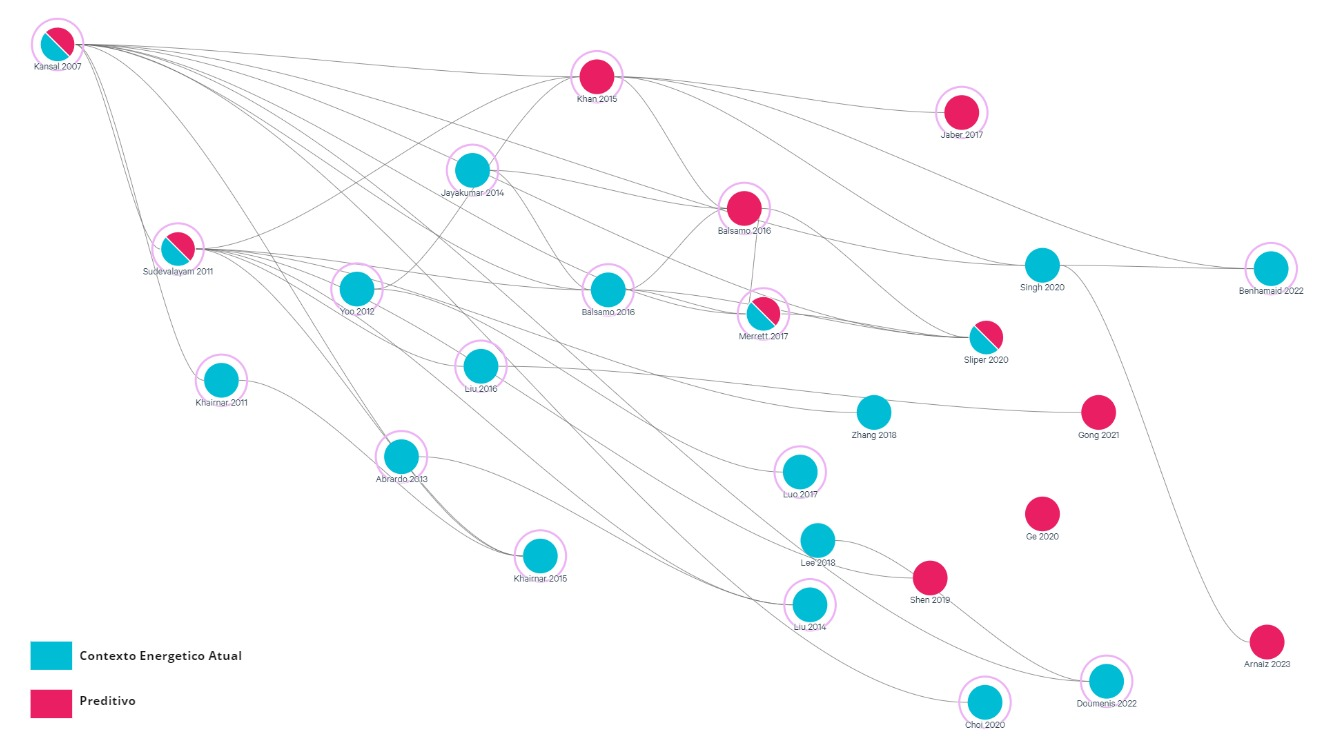
\includegraphics[width=1\linewidth]{Imagens/cap3/divisaodostrabalhos.jpg} 
	
	Fonte: elaborado pelo autor.
\end{figure}

\begin{comment}
\begingroup
\begin{table}[htbp]
	
	\centering
	\caption{ Trabalhos observados.}
	\smaller
	\tabcolsep=0.15cm
	\begin{tabular}{cp{11cm}c}
		\toprule
		ID &  Titulo & Tipo \\\midrule
		SB0-0001 &	Power Management in Energy Harvesting Sensor Networks & Periódico \\
		SB1-0001 &	 Energy-Driven Computing: Rethinking the Design of Energy Harvesting Systems & Conferência\\
		SB1-0002 &	 Lightweight operation scheduling for self-powered IoT devices  & Conferência \\
		SB1-0003 & Adaptive operating mode management model for efficient energy harvesting systems & Periódico\\
		SB1-0004 &	Energy Management in Wireless Sensor Networks: A Survey  &\\
		SB1-0005 &	Discrete-Rate Adaptation and Selection in Energy Harvesting Wireless Systems & \\
		SB1-0006 &	Energy Harvesting Sensor Nodes: Survey and Implications &\\
		SB2-0001 &	Energy-driven computing &\\
		SB2-0002 &	Hibernus++: A Self-Calibrating and Adaptive System for Transiently-Powered Embedded Devices &\\
		SB2-0003 &	Graceful Performance Modulation for Power-Neutral Transient Computing Systems &\\
		SB2-0004 &	Energy management for solar-powered IoT devices with performance adjustment &\\
		SB2-0005 &	Dynamic Duty-Cycle Scheduling Schemes for Energy-Harvesting Wireless Sensor Networks &\\
		SB2-0006 & Recent advances in energy management for Green-IoT: An up-to-date and comprehensive survey &\\
		SB2-0007 & Reducing the Data Transmission in Sensor Networks through Kruskal-Wallis Model &\\
		SB2-0008 & Power and Discrete Rate Adaptation for Energy Harvesting Wireless Nodes  &\\
		SB2-0009 & Adaptive Energy Management by Reinforcement Learning in Cluster-based Solarpowered WSNs& \\
		SB2-0010 & Energy-efficient Activation/Inactivation Strategy for Long-term IoT Network Operation& \\
		SB2-0011 &	 Towards a Perpetual IoT System: Wireless Power Management Policy with Threshold Structure&\\
		SB2-0012 &	Energy Harvesting Wireless Sensor Networks: Delay Analysis Considering Energy Costs of Sensing and Transmission& \\
		SB2-0013 &	Performance of Wireless-Powered Sensor Transmission Considering Energy Cost of Sensing &\\
		SB3-0001 &  Powering the Internet of Things&\\
		SB3-0002 & Optimal sleep time controller based on traffic prediction and residual energy in duty-cycled wireless sensor networks &\\
		SB3-0003 & A survey and taxonomy on energy management schemes in wireless sensor networks& \\
		SB3-0004 & Sleep, Sense or Transmit: Energy-Age Tradeoff for Status Update With Two-Threshold Optimal Policy &\\
		SB3-0005 & A Game Theory Distributed Approach for Energy Optimization in WSNs&\\
		SB4-0001 & Energy and relevance-aware adaptive monitoring method for wireless sensor	nodes with hard energy constraint&\\\midrule
		 
	\end{tabular}
\end{table}
\endgroup
\end{comment}




\begin{comment}

\begingroup
\begin{table}[ht]	
	\centering
	\caption{ Categorização dos Trabalhos.}
	\smaller
	\tabcolsep=0.1cm
	\begin{tabular}{lccccccccccccccccccccccccccc} 
	 & 
\rot{\cite{kansal_power_2007}} &
\rot{\cite{merrett_energy-driven_2017}} &
\rot{\cite{doumenis_lightweight_2022}} &
\rot{\cite{choi_adaptive_2020}} &
\rot{\cite{khan_energy_2015}} &
\rot{\cite{khairnar_discrete-rate_2015}} &
\rot{\cite{sudevalayam_energy_2011}} &
\rot{\cite{sliper_energy-driven_2020}} &
\rot{\cite{balsamo_hibernus_2016}} &
\rot{\cite{balsamo_graceful_2016}} &
\rot{\cite{lee_energy_2018}} &
\rot{\cite{yoo_dynamic_2012}} &
\rot{\cite{benhamaid_recent_2022}} &
\rot{\cite{jaber_reducing_2017}} &
\rot{\cite{khairnar_power_2011}} &
\rot{\cite{ge_adaptive_2020}} &
\rot{\cite{shen_energy-efficient_2019}} &
\rot{\cite{zhang_toward_2018}} &
\rot{\cite{liu_energy_2016}} &
\rot{\cite{liu_performance_2015}} &
\rot{\cite{jayakumar_powering_2014}} &
\rot{\cite{arnaiz_energy_2024}} &
\rot{\cite{singh_survey_2020}} &
\rot{\cite{gong_sleep_2022}} &
\rot{\cite{abrardo_game_2013}} &
\rot{\cite{arnaiz_energy_2024}} \\ \midrule
	
	Conservação & \checkmark & \checkmark & \checkmark & \checkmark & * & *& * & \checkmark & * & *& * & *& \checkmark & *& \checkmark & \checkmark & * & *& * & *& * & *& \checkmark & *& * & \checkmark  \\
	Otimização & \checkmark & \checkmark & * & *& \checkmark & *& * & *& \checkmark & \checkmark& \checkmark & \checkmark& \checkmark & \checkmark& \checkmark & \checkmark & * & *& \checkmark & \checkmark& * & *& * & *& * & * \\
	Previsão & * & *& * & *& * & *& * & *& * & *& * & *& * & *& * & *& * & *& * & *& * & *& * & *& * & *   \\
	\end{tabular}
\end{table}

\end{comment}
\section{Considerações}

A revisão realizada constatou a atenção sobr



 primordial da adequação de comportamento alguns termos utilizados para expressar a ação de adequação de comportamento dos dispositivos, \textit{Adaptative Duty-Cycle}, 
adaptive operating,
lightweight operation scheduling,
traffic patterns,
traffic management,
smoothing factor e
rate-limit, são termos utilizados recorrentemente nos trabalhos para indicar ajuste de comportamento, todavia a área de atuação desses ajustes podem variar conforme contexto. Após \citeonline{kansal_power_2007} apresentar sua teoria de coleta energética, o termo \textit{duty-cycle} foi utilizado para representar os eventos que conduzem o dispositivo a gastar seus recursos energéticos.


 Assim, os trabalhos encontrados abordam o ajuste de comportamento dos dispositivos com fator para sua 



Quais são os efeitos do throttling na vida útil da bateria e na durabilidade dos dispositivos IoT?
Como o throttling pode ser integrado com outras estratégias de gerenciamento de energia, como o duty cycling, para otimizar a disponibilidade e a eficiência energética em sistemas IoT?
Como o throttling pode ser adaptado e otimizado para diferentes tipos de dispositivos IoT e ambientes de operação?
Qual é a eficácia do throttling na melhoria da disponibilidade de sistemas IoT impulsionados por energia?


definem a ação de limitar a operação do dispositivo

%\blindtext[2]